\section{System Model}
\label{sec:model}
%----------------------------------------------------------------------------------------%
\subsection{Network Model}
\begin{figure*}[htp!]
    \centering
    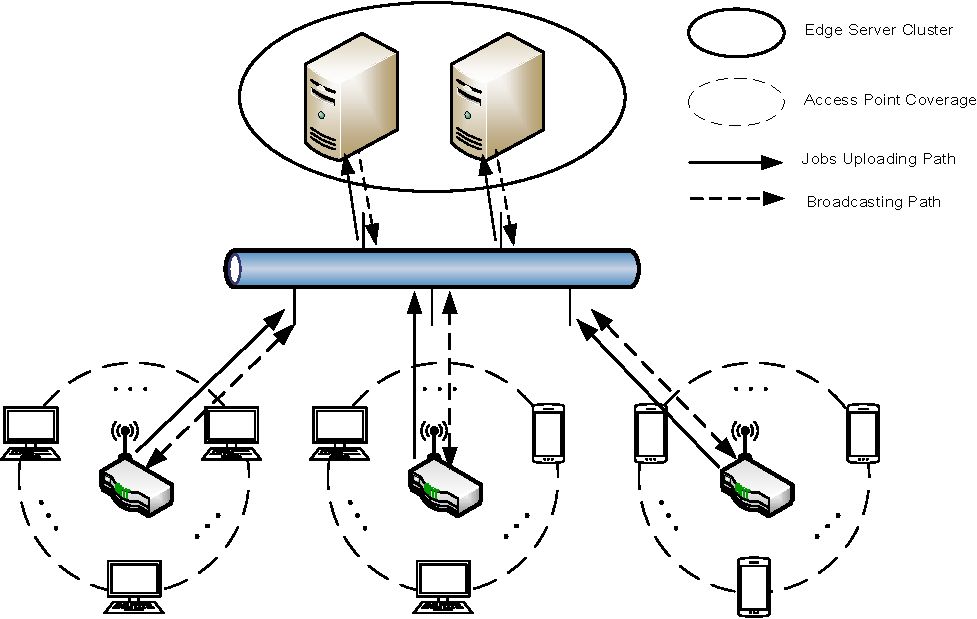
\includegraphics[width=0.80\textwidth]{system-model.pdf}
    \caption{The Illustration of MEC System Model}
    \label{fig:system}
\end{figure*}

We consider an edge computing system with $K$ Access Points (APs) and $M$ edge servers, which are connected in a network as illustrated in Fig.\ref{fig:system}.
The sets of APs and edge servers are denoted as $\apSet \define \set{1,\dots,K}$ and $\esSet \define \set{1,\dots,M}$, respectively.
\comments{
    The communication latency among these APs and edge servers is random.
}
Without loss of generality, it is assumed that there are $J$ types of jobs computed in this system, which are denoted via the set $\mathcal{J} \define \set{1,\dots,J}$.
Each AP collects the computation jobs from the mobile users within its coverage, and makes decision on the processing edge servers for each job type.
It is assumed that the $k$-th AP only dispatches the computation jobs to the edge servers within a certain number of hops.
Let $\esSet_{k} \subseteq \esSet$ be the set of edge servers which can compute the jobs from the $k$-th AP, and $\apSet_{m}$ be the set of APs, which may upload jobs to the $m$-th edge server.
We refer to $\esSet_{k}$ as the \emph{candidate server set} of the $k$-th AP, and $\apSet_{m}$ as the \emph{potential AP set} of the $m$-th edge server ($\forall k\in\apSet, m\in\esSet$).
Different APs may have different candidate servers according to their locations in the network, as illustrated in Fig.\ref{fig:system}.
In this edge computing network, each AP and edge server periodically broadcast their state information (the state information is defined in the Section \ref{subsec:broadcast}), and one AP updates its strategy of job dispatching when receiving the broadcast state information.
In this paper, we shall optimize the job dispatching strategy distributively at APs with partially collected broadcast state information and random broadcast latency.

%NOTE: [job space support and arrival process]
The time axis is organized by time slots.
The job arrivals of the $j$-th job type at the $k$-th AP ($\forall k\in\apSet,j\in\jSpace$) in different time slots are assumed to be independent and identically distributed (i.i.d.) Bernoulli random variables, and the arrival probability is denoted as $\lambda_{k,j}$.
Let $A_{k,j}(t) \in \set{0,1}$ represents the event of job arrival, where $A_{k,j}(t)=1$ means one job of the $j$-th job type arrives at the $k$-th AP in the $t$-th time slot, and $A_{k,j}(t)=0$ means other wise.
Hence,
\begin{align}
    \Pr\{ A_{k,j}(t) = 1 \} = \lambda_{k,j}, \forall t,k\in\apSet,j\in\jSpace.
\end{align}

%NOTE: [uploading process]
Each AP immediately dispatches each type of received jobs to one edge server.
Different types of jobs may have different distributions of the input data size.
Moreover, due to the random traffic in the network, the job uploading from one AP to one edge server consumes a random number of time slots.
It is assumed that the distributions of uploading time are independent for each job.
Specifically, let $\mathbb{U}_{k,m,j}(\Xi)$ be the uploading latency distribution of the $j$-th job type from the $k$-th AP to the $m$-th edge server with support $\set{1, \dots, \Xi}$ ($\forall k\in\apSet, m\in\esSet, j\in\jSpace$).
% In practice, the distribution of uploading latency may not be known to the APs or edge servers in advance.

%NOTE: [processing process]
There are $J$ parallel virtual machines (VMs) running on each edge server for processing the $J$ job types, respectively.
For each job type, the uploaded jobs are computed in a First-Come-First-Serve (FCFS) manner.
Hence, a processing queue with a maximum job number $L_{max}$ is established for each VM.
The arrival jobs will be discarded when the processing queue is full.
Furthermore, we adopt the \emph{unrelated machines assumption} as in \cite{tan-online}.
Specifically, it is assumed that the computation time of different job types on different edge servers follows independent memory-less Geometric distribution with different expectations \cite{TOWC18-HuangKb}.
Let $\mathbb{G}(1/c_{m,j})$ be the distribution of the computation time slots for the $j$-th job type on the $m$-th edge server, where $\mathbb{G}$ denotes the Geometric distribution, and $c_{m,j}$ is the expectation.
Let $f_{m,j}$ be its probability mass function (PMF) and we have:
\begin{align}
    f_{m,j}(k) \define (1-\frac{1}{c_{m,j}})^{k-1} \frac{1}{c_{m,j}}.
\end{align}
%----------------------------------------------------------------------------------------%

\subsection{Periodic Broadcast of State Information}
\label{subsec:broadcast}
In order to facilitate distributive dispatching for the APs, it is assumed that all the APs and edge servers will broadcast their \emph{local state information} (LSI) every $t_B$ time slots.
% as depicted in Fig.\ref{fig:brd-timeline}.
We shall refer to every $t_B$ time slots as a broadcast interval.
At the beginning of each broadcast interval, the LSI of AP and edge server is defined as follows, respectively.

%NOTE: State and Broadcast Information for AP
\begin{definition}[Local State Information of AP]
    Let $R^{(k)}_{m,j,\xi}({t,n}) \in \set{0,1}$ be the number of the $j$-th job type being uploaded from the $k$-th AP to the $m$-th edge server at the $n$-th time slot of the $t$-th interval, which has been delivered for $\xi$ time slots;
    and $\omega_{k,j}(t) \in \esSet_{k}$ be the target edge server for processing of the $j$-th job from the $k$-th AP at the $t$-th broadcast interval.
    % ($\forall k\in\apSet, m\in\esSet, j\in\jSpace, \xi\in(0,\Xi]$)    
    The LSI of the $k$-th AP at the $t$-th broadcast interval is given as follows.
    \begin{align}
        \mathcal{R}_{k}(t) \define \set{\vec{R}^{(k)}_{m,j}(t,0), \omega_{k,j}(t) | \forall m\in\esSet_{k}, j\in\jSpace},
    \end{align}
    where
    $\vec{R}^{(k)}_{m,j}(t,0) \define ( R^{(k)}_{m,j,0}(t,0), \dots, R^{(k)}_{m,j,\Xi}(t,0) )$.
\end{definition}

%NOTE: State and Broadcast Information for Edge Server
\begin{definition}[Local State Information of Edge Servers]
    Let $Q_{m,j}({t,n})$ be the pending number of the $j$-th type job on the $m$-th edge server at the $n$-th time slot in the $t$-th interval ($\forall m\in\esSet, j\in\jSpace$).
    The LSI of the $m$-th edge server at the $t$-th broadcast is defined as follows.
    \begin{align}
        \mathcal{Q}_{m}(t) \define \set{Q_{m,j}(t, 0) | \forall j\in\jSpace}.
    \end{align}
\end{definition}

We refer to \emph{global state information} (GSI) as the aggregation of LSI of all the APs and edge servers, which is defined below.
\begin{definition}[Global State Information]
    The global state information (GSI) of the $t$-th broadcast interval is defined as
    \begin{align}
        \Stat(t) \define
            \Brace{
                \mathcal{R}_{k}(t), \mathcal{Q}_{m}(t) | \forall k\in\apSet, m\in\esSet
            }.
    \end{align}
\end{definition}

%NOTE: Conflict of AP set and partial information definition
\accept{
    As the edge computing network resides in MAN, the propagation delay of LSI in such extensive network is not negligible.
    Thus for the $k$-th AP ($\forall k\in\apSet$), the reception latency of the LSI from the edge servers out of its \emph{candidate server set} $\esSet_{k}$ may be not acceptable.
    To alleviate the impact of information reception latency on decision making, we should leverage the definition of \emph{candidate server set} and \emph{potential AP set}, and only use partial information from GSI for decision making for each AP.
}

Hence, we first define the \emph{conflict AP set} as follows.
\begin{definition}[Conflict AP Set]
    \begin{align}
        \ccSet_{k} \define \bigcup_{m\in\esSet_{k}} \apSet_{m}.
        % \ccSet_{k} \define \set{\forall k' \neq k\in\apSet|\esSet_{k'} \cap \esSet_{k} \neq \emptyset}
    \end{align}
    The \emph{conflict AP set} indicates that the subset of APs whose LSI could affect the decision making for the $k$-th AP.
\end{definition}

\begin{figure}[tp]
    \centering
    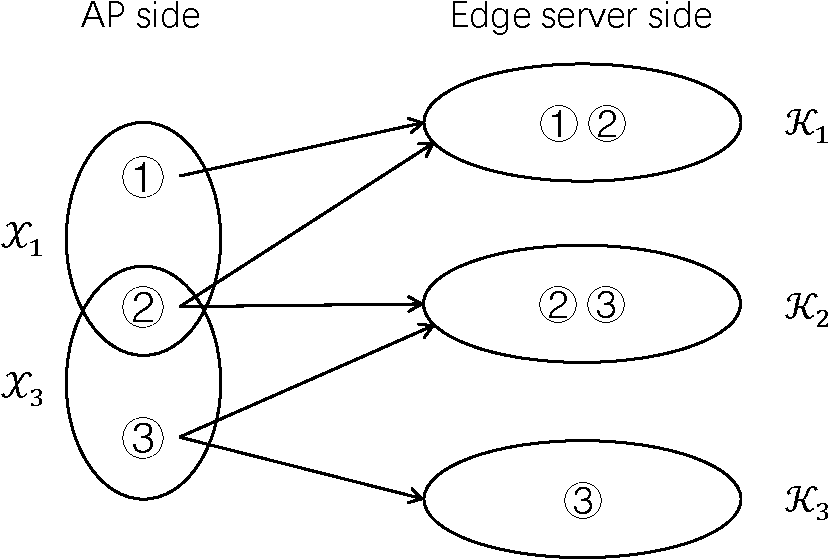
\includegraphics[width=0.45\textwidth]{images/conflict.pdf}
    \caption{The Example Illustration of Conflict Set and Partial Broadcast Information}
    \label{fig:conflict}
\end{figure}

It is assumed that each AP only collect the LSI from the APs in its \emph{conflict AP set} and edge servers from its \emph{candidate server set}.
For a simple example given in Fig.\ref{fig:conflict}, the $1$-st AP only receives LSI from the $2$-nd AP who is in its \emph{conflict AP set}, and LSI from the $1$-st edge server who is in its \emph{candidate server set}.
Hence, we refer to the partial state information as \emph{observed state information} (OSI) and the definition is given as follows.
\begin{definition}[Observed State Information]
    The OSI for the $k$-th AP ($\forall k\in\apSet$) at the $t$-th broadcast is defined as:
    \begin{align}
        \Stat_{k}(t) &\define \set{\mathcal{R}_{k'}(t) | \forall k'\in\ccSet_{k}}
                         \cup \set{\mathcal{Q}_{m}(t) | \forall m\in\esSet_{k}}.
        \label{def:OSI}
    \end{align}
\end{definition}

\begin{figure*}[t]
    \centering
    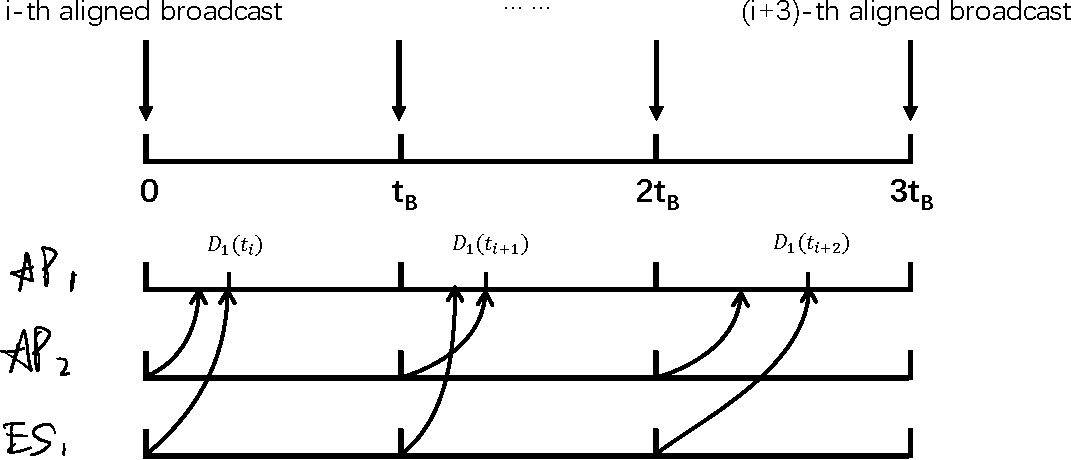
\includegraphics[width=0.80\textwidth]{brd-timeline.pdf}
    \caption{The timeline illustration of reception of OSI for the $1$-st AP with the system setting in Fig.\ref{fig:conflict}.}
    \label{fig:brd-timeline}
\end{figure*}

It is assumed that the $k$-th AP is able to collect its OSI $\mathcal{D}_{k}(t)$ time slots later after the $t$-th broadcast time slot, where $\mathcal{D}_{k}(t)$ is a random variable.
We refer to $\mathcal{D}_{k}(t) \sim \mathbb{D}_{k}(t)$ as the \brlatency~of the $k$-th AP for the $t$-th broadcast with support $\set{1,\dots,t_B}$, i.e. the broadcast interval $t_B$ is set that the $k$-th AP ($\forall k\in\apSet$) could receive the complete OSI before the start of next broadcast interval.

One AP shall update its dispatching decision immediately after the reception of its OSI.
An example is given below to demonstrate the decision changes.
\begin{example}
    In Fig.\ref{fig:brd-timeline} we focus on the decision changes for the $1$-st AP.
    In the $t$-th broadcast interval, it updates its dispatching decisions for all the job type $\mathcal{D}_{1}(t)$ time slots later, which is denoted as $\set{\omega_{1,j}(t) | \forall j\in\jSpace}$.
    At the start of the second broadcast interval, it will firstly keep the the previous decisions unchanged, and then updates the decisions immediately $\mathcal{D}_{1}(t+1)$ time slots later which is denoted as $\set{\omega_{1,j}(t+1) | \forall j\in\jSpace}$.
    And then it repeats the process for the remaining of the time.
\end{example}

%----------------------------------------------------------------------------------------%
%----------------------------------------------------------------------------------------%